\title{B-365 HW 1}
\author{
        Lucas Klein\\
                luklein\\
}
\date{\today}
\documentclass[12pt]{article}
\usepackage{graphicx}

\begin{document}
\maketitle

\section*{Problem 1}
Three  players,  A,B,  and  C,  each  flip  their  coins  until  one  person  has  a different  result  from  the  others. The person having the different coin wins.

\subsection*{(A)}

\paragraph{Answer}
See the .r file. The result was player A won 3255 out of  10000 times.

\subsection*{(B)}

\paragraph{Answer}
$1/\sqrt{n} = 0.01$ , n = 10000

\subsection*{(C)}

\paragraph{Answer}
There is a 95\% chance that p(A wins) is in this interval, this is because I used the vale for 95\% in my calculations.

\subsection*{(D)}
 
 \paragraph{Answer}
 The true probability of an event cannot ever be known because it it would require a running the experiment an infinite number of times to find out.


\section*{Problem 2}
A and B alternate drawing cards from a shuffled pack, replacing each card when done.  A goes first.  Play continues until a heart is drawn.  Simulate this  experiment  to  compute  P(A  draws  first  heart)  to  2  decimal  places($\pm$.005) using the $\sqrt{n}$ rule.

 \paragraph{Answer}
the probability is  0.4967179.
The 95\% interval is from  0.4917556 to 0.5016803.
The half width of the interval is  0.004962316.
See the .r file for the simulation and the calculation code.

\section*{Problem 3}
Two cards are drawn from a shuffled deck.

\subsection*{(A)}

\paragraph{Answer}
The sample space for the experiment is $\Omega=\{(AH,2H), (2H,3H), ... (KC, KS)\}$ or every possible permutation of 2 cards drawn from the deck.
$\|\Omega\| = 2652$

\subsection*{(B)}

\paragraph{Answer}
156 elements

\subsection*{(C)}

\paragraph{Answer}
$156/2652 = 0.05882353$

\section*{Problem 4}
Suppose we are interested in P(A) for some event...

\subsection*{(A)}

\paragraph{Answer}
The out put of running problem 4 in the .r file is bellow:\newline
A occurred 31 out of  300 times\newline
the probability is  0.103333 \newline
The 95\% interval is from 0.06888794 to 0.1377787\newline
The half width of the interval is  0.0344454  \newline

\subsection*{(B)}

\paragraph{Answer}
The plot is emended bellow and can be generated using the method problemFourB() in the .r file.
\begin{center}
	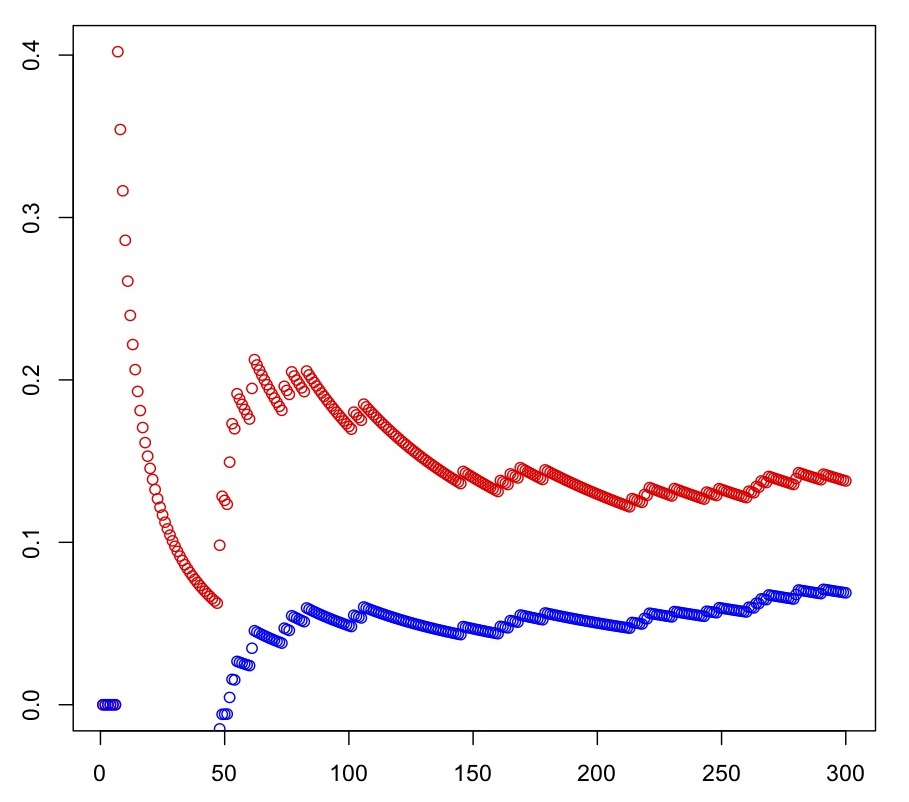
\includegraphics[width=\linewidth]{HW1 prob4 chart.jpg}
\end{center}

\subsection*{(C)}

\paragraph{Answer}
The actual probability was in the interval  0.949 \% of the time. See the method problemFourC() in the .r file.

\section*{Problem 5}
A bag contains n distinct (all different) numbers:\{x1, x2, . . . , xn\}.  Person A draws a number at random, while person B draws a number from the remaining choices.  What is the exact probability that A’s number is greater than B’s number?  Explain your reasoning in detail.

\paragraph{Answer}
The probability is exactly 50\%. This can be seen in in the .r file in the method problemFive(). This is also demonstrated the table bellow. The number of green squares is the same as red squares and so the chance is exactly 50\%.
\begin{center}
	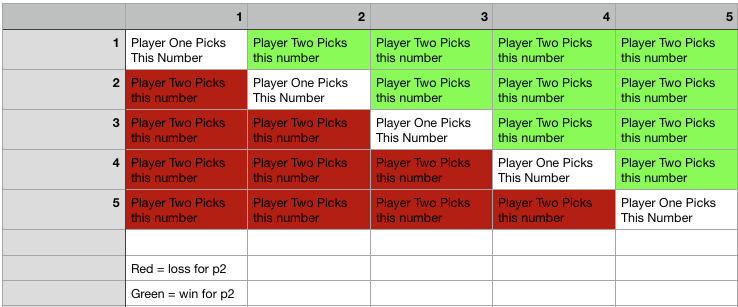
\includegraphics[width=\linewidth]{p5 table.png}
\end{center}

\section*{Problem 6}
Suppose we want to simulate an experiment that can take outcomes...

\paragraph{Answer}
See the .r file for the code.

\end{document}
This is never printed